PacBio okumalarındaki hatalar düzeltildikten sonra genom birleştirme için taslak algoritmamız aşağıda verilmiştir:

Hiperçizge oluşturulması:

\begin{enumerate} 
\item Düzeltilmiş PacBio okumalarındaki bütün k-mer'lere denk gelen düğümlerden oluşan bir çizge oluştur.
\item Her uzun okuma için bir hiperkenar ($E_i$) ekle; öyle ki, $E_i$ sıralanmış (ve tekrarlanabilen) ve uzun okumadaki k-mer'lere denk gelen
bir düğüm kümesi içersin. Burada sıralama k-mer'lerin uzun okumadaki sırası ile belirlensin.
\item Kısa dizi verilerini kullanarak $(k+1)$-mer kenarlarını ekleyerek dizileme kapsamasını geliştir.
\end{enumerate}


Daha sonra algoritmamız Euler yolu bularak genomu birleştirir:

\begin{enumerate}
\item İlk k-mer'i başka bir hiperkenardaki $i$'nci ($i>1$) k-mer olmayan bir hiperkenar ile başla. Böyle bir hiperkenar bulunamazsa herhangi bir hiperkenarı seç.
Bunu ``ana hiperkenar'' olarak belirle.
\item Her aşamada aktif hiperkenarlar listesi tut, öyle ki önekleri (prefix) gezinilmiş yol üzerindeki herhangi bir soneke (suffix) denk gelsin. Bu aşama OLC metotlarına
benzerlik göstermektedir.
\begin{itemize}
\item k-mer'ler ana hiperkenardaki ile aynı sırada takip edilecektir.
\item Eğer aktif listedeki herhangi bir hiperkenar uzaksarsa, bu hiperkenarı aktif listesinden çıkar.
\end{itemize}
\item Ana hiperkenardaki k-mer listesi tamamen kullanıldıktan sonra, aktif listeden yeni hiperkenar seç ve bunu ana hiperkenar olarak belirle.
\item Aktif liste boşalana kadar devam et.
\end{enumerate}

Sıradan hipercizgelerde Euler yolu bulmak NP-zor bir problemdir. Ancak, bizim problemimizde hiperkenarlar sıralı olduğu için doğrusal zamanda çözüleblir. Bu algoritmanın prototip implementasyonu uzun genom bitişikleri oluşturabilmektedir.

{\bf Simulasyon testi:}

Algoritmamızı denemek için 200,447 bp uzunluğunda bir BYK'dan 5X kapsamaya denk gelecek şekilde 325 adet PacBio okuması simüle ettik. Algoritmamızı $k=55$ değeri ile çalıştırdık. Oluşturulan hiperçizge Şekil~\ref{fig:bac-hypergraph}'de verilmiştir. Bu hiperçizge üzerinde bulduğumuz Euler yolu ise biri 196,532 bp, diğeri 757 bp olan iki bitişiği doğru şekilde oluşturmuştur.

\begin{figure}[htb]
  \begin{center}
    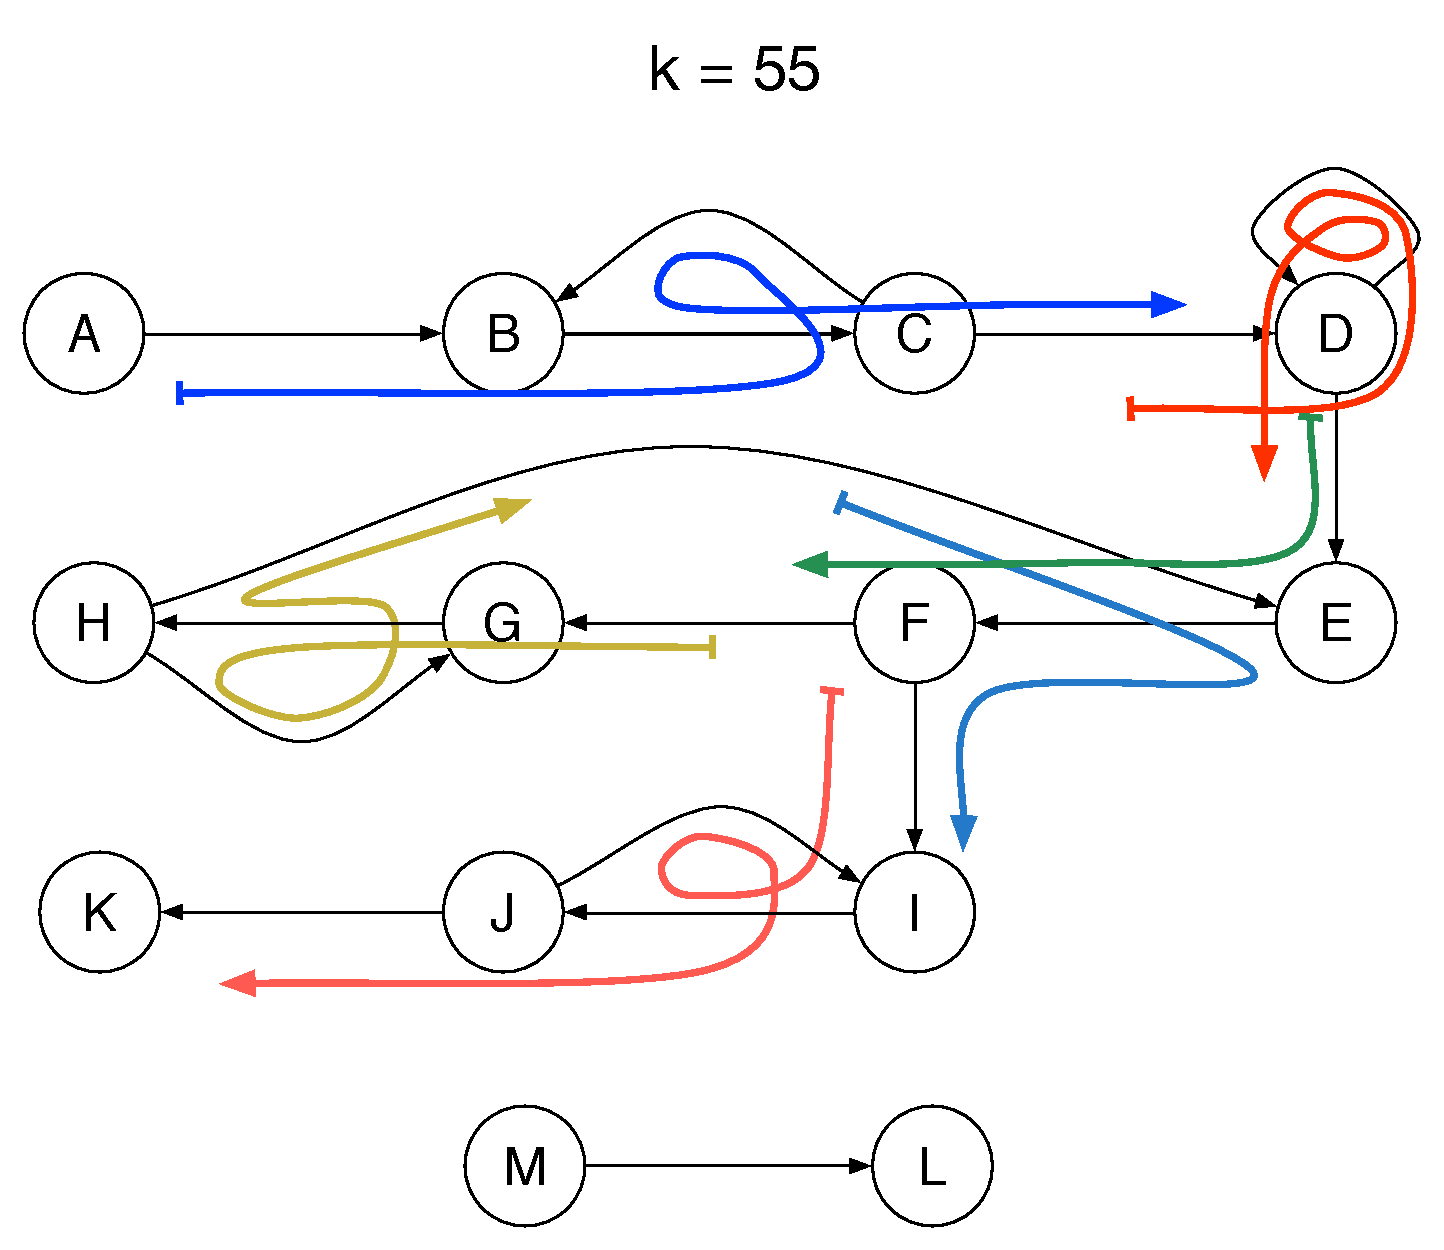
\includegraphics[scale=0.6]{k55.pdf}
  \end{center}
  \caption{Simüle edilmiş BYK verilerinden oluşturulan hiperçizge.}
  \label{fig:bac-hypergraph}
\end{figure}

